\documentclass[aspectratio=169,11pt]{beamer}

\usepackage[T1]{fontenc}
\usepackage[utf8]{inputenc}
\usepackage{lmodern}
\usepackage{amsmath,amssymb,bm}
\usepackage{booktabs}
\usepackage{graphicx}
\usepackage{tikz}
\usepackage{listings}
\usetikzlibrary{arrows.meta,positioning,calc,shapes.geometric}
\graphicspath{{slides/graphics/}{graphics/}}

\definecolor{DeepBlack}{HTML}{050505}
\definecolor{PanelBlack}{HTML}{111111}
\definecolor{SoftBlack}{HTML}{1A1A1A}
\definecolor{Crimson}{HTML}{C8102E}
\definecolor{CrimsonDark}{HTML}{7A0019}
\definecolor{CrimsonSoft}{HTML}{F04B5F}
\definecolor{WarmWhite}{HTML}{F8F7F4}
\definecolor{MutedWhite}{HTML}{CFCFCF}
\definecolor{LineGrey}{HTML}{4B4B4B}

\setbeamercolor{background canvas}{bg=DeepBlack}
\setbeamercolor{normal text}{fg=WarmWhite,bg=DeepBlack}
\setbeamercolor{frametitle}{fg=WarmWhite,bg=DeepBlack}
\setbeamercolor{title}{fg=WarmWhite}
\setbeamercolor{subtitle}{fg=MutedWhite}
\setbeamercolor{structure}{fg=Crimson}
\setbeamercolor{item}{fg=CrimsonSoft}
\setbeamercolor{subitem}{fg=CrimsonSoft}
\setbeamercolor{block title}{fg=WarmWhite,bg=CrimsonDark}
\setbeamercolor{block body}{fg=WarmWhite,bg=PanelBlack}
\setbeamercolor{alerted text}{fg=CrimsonSoft}

\setbeamertemplate{navigation symbols}{}
\setbeamertemplate{itemize item}{\raise0.15ex\hbox{\tiny$\blacktriangleright$}}
\setbeamertemplate{itemize subitem}{\raise0.15ex\hbox{\tiny$\circ$}}

\setbeamerfont{title}{size=\LARGE,series=\bfseries}
\setbeamerfont{subtitle}{size=\large}
\setbeamerfont{frametitle}{size=\Large,series=\bfseries}
\setbeamerfont{footline}{size=\scriptsize}

\newcommand{\icrarlogo}{ICRARJointVenturePartners-black-background-colour-ICRAR.png}
\newcommand{\accentline}{\vspace{-0.2cm}\textcolor{Crimson}{\rule{\linewidth}{1.2pt}}\vspace{0.15cm}}
\newcommand{\redtag}[1]{\tikz[baseline=(x.base)]{\node[fill=CrimsonDark,draw=Crimson,rounded corners=1pt,inner xsep=5pt,inner ysep=2pt](x){\footnotesize\bfseries #1};}}
\newcommand{\tightlist}{\setlength{\itemsep}{0.35em}}
\newcommand{\boxeq}[1]{%
  \begin{center}
  \begin{tikzpicture}
    \node[
      draw=Crimson,
      fill=PanelBlack,
      rounded corners=2pt,
      line width=0.8pt,
      inner xsep=14pt,
      inner ysep=10pt,
      text=WarmWhite
    ] {\large #1};
  \end{tikzpicture}
  \end{center}
}

\setbeamertemplate{frametitle}{%
  \vspace{0.25cm}
  \hspace{0.55cm}%
  \begin{beamercolorbox}[wd=\dimexpr\paperwidth-1.1cm\relax]{frametitle}
    \insertframetitle%
  \end{beamercolorbox}%
  \hspace{0.55cm}\textcolor{Crimson}{\rule{0.88\paperwidth}{1.1pt}}
}

\setbeamertemplate{footline}{%
  \leavevmode
  \hbox to \paperwidth{%
    \hspace{0.55cm}%
    \usebeamerfont{footline}\textcolor{MutedWhite}{Simulation-Based Inference in Astrophysics}%
    \hfill
    \usebeamerfont{footline}\textcolor{MutedWhite}{\insertframenumber/\inserttotalframenumber}%
    \hspace{0.55cm}%
  }%
  \vskip2pt%
}

\lstdefinestyle{python-dark}{
  language=Python,
  basicstyle=\ttfamily\scriptsize\color{WarmWhite},
  keywordstyle=\color{CrimsonSoft}\bfseries,
  stringstyle=\color{MutedWhite},
  commentstyle=\color{LineGrey},
  showstringspaces=false,
  backgroundcolor=\color{PanelBlack},
  frame=single,
  rulecolor=\color{CrimsonDark},
  xleftmargin=0.6em,
  xrightmargin=0.6em,
  aboveskip=0.6em,
  belowskip=0.2em
}

\title{Simulation-Based Inference in Astrophysics}
\subtitle{Bayesian inference when the simulator is easier than the likelihood}
\author{Connor Bottrell}
\institute{ICRAR - International Centre for Radio Astronomy Research}
\date{}

\begin{document}

{
\setbeamertemplate{footline}{}
\begin{frame}
  \begin{tikzpicture}[remember picture,overlay]
    \fill[DeepBlack] (current page.south west) rectangle (current page.north east);
    \draw[Crimson,line width=2.2pt] ([xshift=0.55cm,yshift=-0.55cm]current page.north west)
      rectangle ([xshift=-0.55cm,yshift=0.55cm]current page.south east);
    \fill[CrimsonDark] ([xshift=0.55cm,yshift=-1.65cm]current page.north west)
      rectangle ([xshift=8.9cm,yshift=-1.75cm]current page.north west);
    \node[anchor=south east,inner sep=0pt] at ([xshift=-0.75cm,yshift=0.75cm]current page.south east)
      {\includegraphics[width=4.2cm]{\icrarlogo}};
  \end{tikzpicture}

  \vspace{1.2cm}
  {\usebeamerfont{title}\inserttitle\par}
  \vspace{0.28cm}
  {\usebeamerfont{subtitle}\textcolor{MutedWhite}{\insertsubtitle}\par}
  \vspace{0.75cm}
  \redtag{Python workshop}
  \hspace{0.25cm}
  \redtag{Forward models}
  \hspace{0.25cm}
  \redtag{Likelihood-free inference}

  \vfill
  {\large \insertauthor}\\[0.1cm]
  {\small \textcolor{MutedWhite}{\insertinstitute}}
\end{frame}
}

\begin{frame}{The Problem We Keep Meeting}
  \begin{columns}[T,onlytextwidth]
    \begin{column}{0.52\textwidth}
      \begin{itemize}\tightlist
        \item Astrophysics is full of inverse problems.
        \item We can often simulate the data-generating process.
        \item The corresponding likelihood may be unavailable, unstable, or too expensive.
        \item SBI asks: can simulations teach us the inverse map?
      \end{itemize}
    \end{column}
    \begin{column}{0.43\textwidth}
      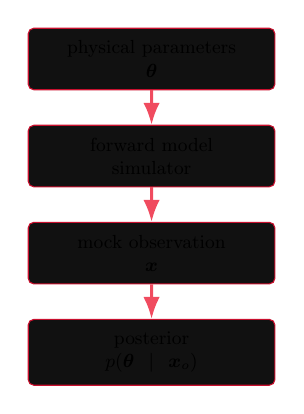
\begin{tikzpicture}[
        scale=0.76,
        transform shape,
        node distance=0.58cm,
        every node/.style={font=\small},
        box/.style={draw=Crimson,fill=PanelBlack,rounded corners=2pt,text width=3.7cm,align=center,inner sep=6pt},
        arr/.style={-Latex,CrimsonSoft,line width=1.1pt}
      ]
        \node[box] (theta) {physical parameters\\$\bm{\theta}$};
        \node[box,below=of theta] (sim) {forward model\\simulator};
        \node[box,below=of sim] (data) {mock observation\\$\bm{x}$};
        \node[box,below=of data] (infer) {posterior\\$p(\bm{\theta}\mid\bm{x}_o)$};
        \draw[arr] (theta) -- (sim);
        \draw[arr] (sim) -- (data);
        \draw[arr] (data) -- (infer);
      \end{tikzpicture}
    \end{column}
  \end{columns}
\end{frame}

\begin{frame}{Workshop Goals}
  \begin{block}{By the end, participants should be able to}
    \begin{itemize}\tightlist
      \item identify the prior, simulator, observation, and posterior target;
      \item explain what makes a likelihood hard to evaluate explicitly;
      \item train a neural posterior estimator from simulations;
      \item interpret posterior samples, degeneracies, and uncertainty;
      \item test the posterior using posterior predictive checks;
      \item explain why an accurate forward model is not optional.
    \end{itemize}
  \end{block}
\end{frame}

\begin{frame}{Bayes' Theorem Is Still The Target}
  \boxeq{$\displaystyle p(\bm{\theta}\mid\bm{x}_o) =
  \frac{p(\bm{x}_o\mid\bm{\theta})\,p(\bm{\theta})}{p(\bm{x}_o)}$}

  \vspace{0.2cm}
  \begin{columns}[T,onlytextwidth]
    \begin{column}{0.31\textwidth}
      \redtag{prior}\\[0.25cm]
      \small What parameter values are plausible before seeing this data?
    \end{column}
    \begin{column}{0.31\textwidth}
      \redtag{likelihood}\\[0.25cm]
      \small How probable is the observed data under a candidate parameter value?
    \end{column}
    \begin{column}{0.31\textwidth}
      \redtag{posterior}\\[0.25cm]
      \small Which parameter values remain plausible after seeing the data?
    \end{column}
  \end{columns}
\end{frame}

\begin{frame}{What Makes The Likelihood Difficult?}
  \begin{block}{A likelihood is not just a goodness-of-fit score}
    \small It is a normalized probability density for the observed data,
    including every stochastic step between parameters and measurement.
  \end{block}

  \vspace{0.25cm}
  \begin{itemize}\tightlist
    \item Detector noise may be non-Gaussian, non-stationary, or poorly characterized.
    \item Selection effects can depend on detection pipelines and survey strategy.
    \item Nuisance variables may require high-dimensional marginalization.
    \item Observations may be indirect summaries rather than direct states.
    \item Simulations may include branching logic, thresholds, and numerical solvers.
    \item Some models are implicit: we can sample $\bm{x}\sim p(\bm{x}\mid\bm{\theta})$, but cannot evaluate $p(\bm{x}\mid\bm{\theta})$.
  \end{itemize}
\end{frame}

\begin{frame}{Astrophysical Examples}
  \begin{columns}[T,onlytextwidth]
    \begin{column}{0.49\textwidth}
      \begin{block}{Likelihoods get awkward when}
        \begin{itemize}\tightlist
          \item the data are sparse Fourier samples;
          \item the noise model is learned empirically;
          \item a catalog was produced by a complex detection algorithm;
          \item the observable is a nonlinear summary statistic;
          \item the model includes subgrid physics or approximate numerics.
        \end{itemize}
      \end{block}
    \end{column}
    \begin{column}{0.49\textwidth}
      \begin{block}{Common SBI candidates}
        \begin{itemize}\tightlist
          \item gravitational-wave strain recovery;
          \item VLBI black-hole imaging;
          \item galaxy population synthesis;
          \item strong lensing image analysis;
          \item cosmological fields and summaries;
          \item transient classification and rates.
        \end{itemize}
      \end{block}
    \end{column}
  \end{columns}
\end{frame}

\begin{frame}{Simulation-Based Inference}
  \begin{block}{The key substitution}
    Instead of evaluating $p(\bm{x}_o\mid\bm{\theta})$, we generate many
    paired examples $(\bm{\theta}, \bm{x})$ and learn an inference object
    from them.
  \end{block}

  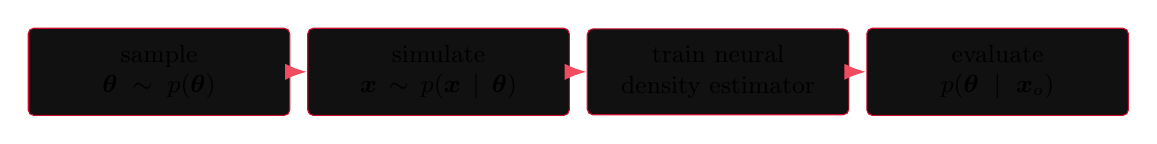
\begin{tikzpicture}[
    every node/.style={font=\small},
    box/.style={draw=Crimson,fill=PanelBlack,rounded corners=2pt,text width=2.9cm,align=center,inner sep=6pt},
    arr/.style={-Latex,CrimsonSoft,line width=1.1pt}
  ]
    \node[box] (prior) at (0,0) {sample\\$\bm{\theta}\sim p(\bm{\theta})$};
    \node[box] (sim) at (3.55,0) {simulate\\$\bm{x}\sim p(\bm{x}\mid\bm{\theta})$};
    \node[box] (train) at (7.1,0) {train neural\\density estimator};
    \node[box] (post) at (10.65,0) {evaluate\\$p(\bm{\theta}\mid\bm{x}_o)$};
    \draw[arr] (prior) -- (sim);
    \draw[arr] (sim) -- (train);
    \draw[arr] (train) -- (post);
  \end{tikzpicture}

  \vspace{0.25cm}
  \small The posterior is still Bayesian. The difference is how we obtain an
  approximation to it.
\end{frame}

\begin{frame}{Three SBI Families}
  \begin{columns}[T,onlytextwidth]
    \begin{column}{0.32\textwidth}
      \begin{block}{NPE}
        \small Neural posterior estimation learns
        \[
          q_\phi(\bm{\theta}\mid\bm{x})
        \]
        directly.
      \end{block}
    \end{column}
    \begin{column}{0.32\textwidth}
      \begin{block}{NLE}
        \small Neural likelihood estimation learns
        \[
          q_\phi(\bm{x}\mid\bm{\theta})
        \]
        then samples the posterior.
      \end{block}
    \end{column}
    \begin{column}{0.32\textwidth}
      \begin{block}{NRE}
        \small Neural ratio estimation learns a likelihood-to-evidence ratio
        \[
          r_\phi(\bm{x},\bm{\theta}).
        \]
      \end{block}
    \end{column}
  \end{columns}

  \vspace{0.35cm}
  \small In this workshop we use \alert{NPE}: it is intuitive, amortized, and
  gives posterior samples quickly once trained.
\end{frame}

\begin{frame}{Neural Posterior Estimation}
  \begin{block}{Training objective}
    \[
      \hat{\phi}
      =
      \arg\max_\phi
      \sum_{i=1}^{N}
      \log q_\phi(\bm{\theta}_i\mid \bm{x}_i),
      \qquad
      \bm{\theta}_i\sim p(\bm{\theta}),\quad
      \bm{x}_i\sim p(\bm{x}\mid\bm{\theta}_i).
    \]
  \end{block}

  \begin{itemize}\tightlist
    \item The density estimator learns a conditional distribution, not a point estimate.
    \item It can represent degeneracies and non-Gaussian posterior shapes.
    \item After training, one model can be conditioned on many observations.
    \item The result is approximate and must be checked.
  \end{itemize}
\end{frame}

\begin{frame}[fragile]{The Workflow In Python}
  \begin{lstlisting}[style=python-dark]
prior = BoxUniform(low, high)

theta = prior.sample((num_simulations,))
x = simulator(theta)

inference = NPE(prior=prior)
density_estimator = inference.append_simulations(theta, x).train()
posterior = inference.build_posterior(density_estimator)

samples = posterior.sample((5000,), x=x_observed)
  \end{lstlisting}

  \vspace{0.15cm}
  \begin{block}{Everything hangs on the simulator}
    The code is short because the scientific work is hidden inside the forward
    model: how parameters become mock observations.
  \end{block}
\end{frame}

\begin{frame}{The Forward Model Is The Scientific Claim}
  \begin{columns}[T,onlytextwidth]
    \begin{column}{0.58\textwidth}
      \begin{itemize}\tightlist
        \item SBI does not make the simulator true.
        \item It learns the posterior implied by the simulator and prior.
        \item If the simulator omits a relevant physical or instrumental effect,
        the posterior can be precise and wrong.
        \item Forward-model validation is therefore part of inference, not a
        separate housekeeping task.
      \end{itemize}
    \end{column}
    \begin{column}{0.38\textwidth}
      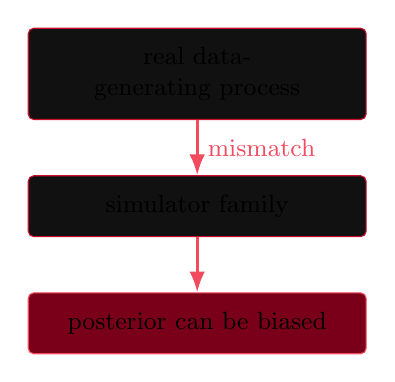
\begin{tikzpicture}[
        every node/.style={font=\small},
        box/.style={draw=Crimson,fill=PanelBlack,rounded corners=2pt,text width=3.8cm,align=center,inner sep=7pt},
        bad/.style={draw=CrimsonSoft,fill=CrimsonDark,rounded corners=2pt,text width=3.8cm,align=center,inner sep=7pt}
      ]
        \node[box] (truth) {real data-generating process};
        \node[box,below=0.7cm of truth] (model) {simulator family};
        \node[bad,below=0.7cm of model] (post) {posterior can be biased};
        \draw[-Latex,CrimsonSoft,line width=1.0pt] (truth) -- node[right]{mismatch} (model);
        \draw[-Latex,CrimsonSoft,line width=1.0pt] (model) -- (post);
      \end{tikzpicture}
    \end{column}
  \end{columns}
\end{frame}

\begin{frame}{What Must The Simulator Include?}
  \begin{columns}[T,onlytextwidth]
    \begin{column}{0.49\textwidth}
      \begin{block}{Physical model}
        \begin{itemize}\tightlist
          \item source parameters;
          \item emission or waveform physics;
          \item cosmological and environmental effects;
          \item population-level variability.
        \end{itemize}
      \end{block}
    \end{column}
    \begin{column}{0.49\textwidth}
      \begin{block}{Measurement model}
        \begin{itemize}\tightlist
          \item instrument response;
          \item noise and calibration uncertainty;
          \item selection function;
          \item data reduction and summaries.
        \end{itemize}
      \end{block}
    \end{column}
  \end{columns}

  \vspace{0.35cm}
  \boxeq{$\text{good SBI} = \text{good prior} + \text{good simulator} + \text{good diagnostics}$}
\end{frame}

\begin{frame}{Priors Are Part Of The Model}
  \begin{itemize}\tightlist
    \item The training distribution is usually the prior.
    \item The neural estimator sees many more examples in high-prior-volume regions.
    \item A broad prior can waste simulations in irrelevant regions.
    \item A narrow prior can exclude the truth.
    \item Sequential SBI can concentrate simulations near a particular observation, but must handle proposal corrections carefully.
  \end{itemize}

  \vspace{0.35cm}
  \begin{block}{Workshop habit}
    Plot prior predictive simulations before training. If the simulations do not
    look like plausible observations, fix the simulator or the prior first.
  \end{block}
\end{frame}

\begin{frame}{Compression And Summary Statistics}
  \begin{block}{The observation may be high-dimensional}
    Time series, images, spectra, catalogs, and maps can be much larger than the
    parameter vector.
  \end{block}

  \begin{itemize}\tightlist
    \item Use the full data when the density estimator can handle it.
    \item Use learned embeddings, summary networks, or physically motivated summaries when needed.
    \item Avoid summaries that erase information about parameters of interest.
    \item Test compression by checking posterior recovery on simulated data with known truth.
  \end{itemize}
\end{frame}

\begin{frame}{Diagnostics: Trust But Verify}
  \begin{columns}[T,onlytextwidth]
    \begin{column}{0.49\textwidth}
      \begin{block}{Posterior diagnostics}
        \begin{itemize}\tightlist
          \item marginal and joint posterior plots;
          \item simulation-based calibration;
          \item coverage tests;
          \item sensitivity to simulation budget;
          \item prior sensitivity checks.
        \end{itemize}
      \end{block}
    \end{column}
    \begin{column}{0.49\textwidth}
      \begin{block}{Posterior predictive checks}
        \begin{itemize}\tightlist
          \item draw $\bm{\theta}^{(s)}\sim p(\bm{\theta}\mid\bm{x}_o)$;
          \item simulate $\bm{x}^{(s)}\sim p(\bm{x}\mid\bm{\theta}^{(s)})$;
          \item compare simulated data to the observed data;
          \item look for systematic residual structure.
        \end{itemize}
      \end{block}
    \end{column}
  \end{columns}
\end{frame}

\begin{frame}{Worked Example: Noisy Chirp Recovery}
  \begin{columns}[T,onlytextwidth]
    \begin{column}{0.48\textwidth}
      \begin{block}{Parameters}
        \begin{itemize}\tightlist
          \item chirp mass;
          \item amplitude;
          \item merger time;
          \item phase.
        \end{itemize}
      \end{block}
    \end{column}
    \begin{column}{0.48\textwidth}
      \begin{block}{Observation}
        \begin{itemize}\tightlist
          \item one noisy strain segment;
          \item colored Gaussian noise;
          \item compact, inspectable simulator;
          \item posterior predictive waveform overlay.
        \end{itemize}
      \end{block}
    \end{column}
  \end{columns}

  \vspace{0.35cm}
  \small This is deliberately not a production waveform. It is a transparent
  sandbox for learning SBI before moving to domain-grade tools.
\end{frame}

\begin{frame}{Chirp Recovery As An SBI Graph}
  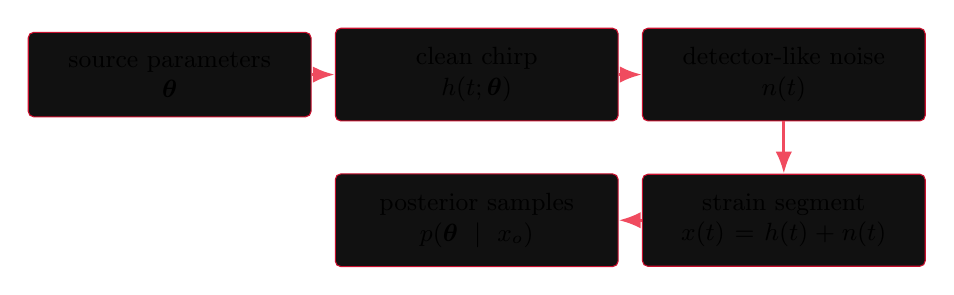
\begin{tikzpicture}[
    every node/.style={font=\small},
    box/.style={draw=Crimson,fill=PanelBlack,rounded corners=2pt,text width=3.1cm,align=center,inner sep=7pt},
    arr/.style={-Latex,CrimsonSoft,line width=1.1pt}
  ]
    \node[box] (theta) at (0,0.8) {source parameters\\$\bm{\theta}$};
    \node[box] (wave) at (3.9,0.8) {clean chirp\\$h(t;\bm{\theta})$};
    \node[box] (noise) at (7.8,0.8) {detector-like noise\\$n(t)$};
    \node[box] (obs) at (7.8,-1.05) {strain segment\\$x(t)=h(t)+n(t)$};
    \node[box] (post) at (3.9,-1.05) {posterior samples\\$p(\bm{\theta}\mid x_o)$};
    \draw[arr] (theta) -- (wave);
    \draw[arr] (wave) -- (noise);
    \draw[arr] (noise) -- (obs);
    \draw[arr] (obs) -- (post);
  \end{tikzpicture}

  \vspace{0.35cm}
  \begin{block}{Teaching moment}
    The posterior width is not just a neural-network artifact. It reflects noise,
    parameter degeneracy, prior support, and simulator adequacy.
  \end{block}
\end{frame}

\begin{frame}{Optional Extension: Sparse VLBI Ring}
  \begin{block}{A different observation model}
    VLBI does not observe the image directly. It samples sparse Fourier
    components of the sky brightness distribution.
  \end{block}

  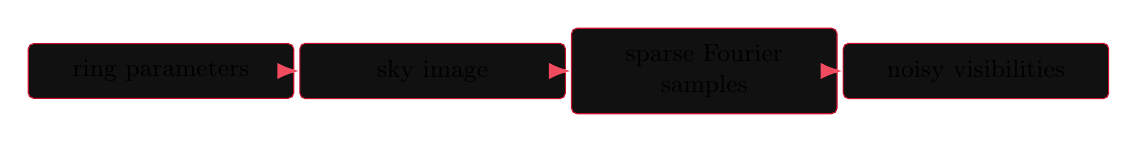
\begin{tikzpicture}[
    every node/.style={font=\small},
    box/.style={draw=Crimson,fill=PanelBlack,rounded corners=2pt,text width=2.95cm,align=center,inner sep=6pt},
    arr/.style={-Latex,CrimsonSoft,line width=1.1pt}
  ]
    \node[box] (theta) at (0,0) {ring parameters};
    \node[box] (image) at (3.45,0) {sky image};
    \node[box] (uv) at (6.9,0) {sparse Fourier samples};
    \node[box] (data) at (10.35,0) {noisy visibilities};
    \draw[arr] (theta) -- (image);
    \draw[arr] (image) -- (uv);
    \draw[arr] (uv) -- (data);
  \end{tikzpicture}

  \vspace{0.35cm}
  \small The SBI logic is unchanged, but the forward model now includes the
  measurement operator and the sparsity pattern.
\end{frame}

\begin{frame}{Why Sparsity Matters}
  \begin{itemize}\tightlist
    \item Many images can agree with the same sparse visibility measurements.
    \item The posterior may constrain ring diameter while leaving asymmetry broad.
    \item Regularization, priors, and model class become scientifically visible.
    \item SBI can expose these degeneracies as posterior uncertainty rather than hiding them in one reconstruction.
  \end{itemize}

  \vspace{0.35cm}
  \begin{block}{Careful language}
    A toy ring model can teach sparse inverse problems. It should not be sold as
    reproducing the full Event Horizon Telescope imaging analysis.
  \end{block}
\end{frame}

\begin{frame}{Failure Modes}
  \begin{columns}[T,onlytextwidth]
    \begin{column}{0.49\textwidth}
      \begin{block}{Scientific failure}
        \begin{itemize}\tightlist
          \item missing physics;
          \item wrong noise model;
          \item unmodeled selection;
          \item prior excludes plausible truth;
          \item summaries remove key information.
        \end{itemize}
      \end{block}
    \end{column}
    \begin{column}{0.49\textwidth}
      \begin{block}{Computational failure}
        \begin{itemize}\tightlist
          \item too few simulations;
          \item poor neural density architecture;
          \item unstable normalization;
          \item extrapolation outside training support;
          \item no calibration check.
        \end{itemize}
      \end{block}
    \end{column}
  \end{columns}
\end{frame}

\begin{frame}{Practical Recipe}
  \begin{enumerate}
    \item Write down $\bm{\theta}$, $\bm{x}$, and the posterior target.
    \item Choose a prior with defensible support.
    \item Build the simplest forward model that produces realistic mock data.
    \item Plot prior predictive simulations.
    \item Train an SBI estimator with a modest simulation budget.
    \item Check inference on simulated observations with known truth.
    \item Apply to the real observation.
    \item Run posterior predictive checks and stress tests.
  \end{enumerate}
\end{frame}

\begin{frame}{How To Read A Posterior Plot}
  \begin{itemize}\tightlist
    \item Narrow marginal: parameter is well constrained under the model.
    \item Wide marginal: data, prior, or simulator do not identify it strongly.
    \item Curved contour: nonlinear degeneracy.
    \item Boundary pile-up: prior edge or model mismatch may matter.
    \item Truth outside credible region in simulated tests: calibration problem.
  \end{itemize}

  \vspace{0.35cm}
  \begin{block}{Workshop phrase}
    The posterior is not a trophy. It is a compressed diagnostic of assumptions,
    data quality, and identifiability.
  \end{block}
\end{frame}

\begin{frame}{Live Notebook Structure}
  \begin{columns}[T,onlytextwidth]
    \begin{column}{0.49\textwidth}
      \begin{block}{Notebook 1}
        \begin{itemize}\tightlist
          \item simulate noisy chirps;
          \item train NPE;
          \item infer one observation;
          \item overlay posterior predictive waveforms;
          \item add a glitch and diagnose mismatch.
        \end{itemize}
      \end{block}
    \end{column}
    \begin{column}{0.49\textwidth}
      \begin{block}{Notebook 2}
        \begin{itemize}\tightlist
          \item simulate a toy ring image;
          \item measure sparse visibilities;
          \item infer ring parameters;
          \item visualize posterior image draws;
          \item vary uv sparsity.
        \end{itemize}
      \end{block}
    \end{column}
  \end{columns}
\end{frame}

\begin{frame}{Discussion Prompts}
  \begin{itemize}\tightlist
    \item What part of the forward model would you trust least?
    \item Which parameters are actually identifiable from the observation?
    \item How would you validate the simulator before using real data?
    \item What summaries would you choose if the raw data were too large?
    \item How would selection effects enter the simulator?
    \item What posterior predictive mismatch would make you stop?
  \end{itemize}
\end{frame}

\begin{frame}{Takeaways}
  \begin{block}{The SBI mindset}
    \begin{itemize}\tightlist
      \item Start from Bayes, not from a neural network.
      \item Use simulations when likelihood evaluation is the hard part.
      \item Treat the simulator as the central scientific object.
      \item Prefer posterior distributions over point estimates.
      \item Check calibration and posterior predictive behavior.
      \item Be explicit about what the model can and cannot explain.
    \end{itemize}
  \end{block}

  \vspace{0.3cm}
  \centering
  \redtag{simulate forward}
  \hspace{0.2cm}
  \redtag{infer backward}
  \hspace{0.2cm}
  \redtag{validate always}
\end{frame}

{
\setbeamertemplate{footline}{}
\begin{frame}
  \begin{tikzpicture}[remember picture,overlay]
    \fill[DeepBlack] (current page.south west) rectangle (current page.north east);
    \draw[Crimson,line width=2.2pt] ([xshift=0.55cm,yshift=-0.55cm]current page.north west)
      rectangle ([xshift=-0.55cm,yshift=0.55cm]current page.south east);
    \node[anchor=south east,inner sep=0pt] at ([xshift=-0.75cm,yshift=0.75cm]current page.south east)
      {\includegraphics[width=4.2cm]{\icrarlogo}};
  \end{tikzpicture}
  \vspace{2.25cm}
  {\Huge\bfseries Questions}\\[0.45cm]
  {\large \textcolor{MutedWhite}{What simulator would you trust enough to invert?}}\\[0.75cm]
  \redtag{Bayes}
  \hspace{0.2cm}
  \redtag{SBI}
  \hspace{0.2cm}
  \redtag{Astrophysics}
\end{frame}
}

\end{document}
